\documentclass[letterpaper,11pt]{article}
\oddsidemargin -1.0cm \textwidth 17.5cm

\usepackage[utf8]{inputenc}
\usepackage[activeacute,spanish, es-lcroman]{babel}
\decimalpoint
\usepackage{amsfonts,setspace}
\usepackage{amsmath}
\usepackage{amssymb, amsmath, amsthm}
\usepackage{comment}
\usepackage{float}
\usepackage{amssymb}
\usepackage{dsfont}
\usepackage{anysize}
\usepackage{multicol}
\usepackage{enumerate}
\usepackage{graphicx}
\usepackage[left=1.5cm,top=2cm,right=1.5cm, bottom=1.7cm]{geometry}
\setlength\headheight{1.5em} 
\usepackage{fancyhdr}
\usepackage{multicol}
\usepackage{hyperref}
\usepackage{wrapfig}
\usepackage{subcaption}
\usepackage{siunitx}
\usepackage{cancel}
\usepackage{mdwlist}
\usepackage{svg}
\pagestyle{fancy}
\fancyhf{}
\renewcommand{\labelenumi}{\normalsize\bfseries P\arabic{enumi}.}
\renewcommand{\labelenumii}{\normalsize\bfseries (\alph{enumii})}
\renewcommand{\labelenumiii}{\normalsize\bfseries \roman{enumiii})}


\begin{document}
\rfoot[]{pág. \thepage}

\begin{center}
	\LARGE\textbf{Gravitación}
\end{center}

\vspace{-1cm}
\begin{enumerate}\setlength{\itemsep}{0.4cm}

\item[]

\item Cierto sistema estelar cuaternario consiste en tres estrellas, cada una de masa $m$, que se mueven en la misma órbita circular de radio $r$ en torno a una estrella central de masa $M$. Las estrellas orbitan en el mismo sentido y se ubican a un tercio de revolución una de otra. Demuestre que el periodo de cada una de las tres estrellas es

$$T = 2\pi \sqrt{\frac{r^3}{G \left(M + m / \sqrt{3} \right)}}$$

\item Dos satélites artificiales de igual masa orbitan alrededor de un planeta. $S_1$ se mueve en una órbita circular de radio $10^8\SI{}{\meter}$ y periodo de $5$ días, $S_2$ se mueve en una órbita elíptica de radios $r_{min} = 10^8\SI{}{\meter}$ y $r_{max}~=~2~\cdot~10^8\SI{}{\meter}$

\begin{multicols}{2}
    \begin{enumerate}
        \item A partir de los datos para la órbita circular, calcule la masa del planeta
        \item Encuentre el periodo de $S_2$
        \item ¿Cuál satélite es más veloz al pasar por $B$? ¿Cuál tiene mayor energía?
        \item Calcule el cuociente entre las velocidades que $S_2$ tiene en $B$ y en $A$
        \item ¿Qué maniobra debería ordenar el puesto de mando para poner $S_2$ en la órbita de $S_1$?
    \end{enumerate}

    \columnbreak

    \begin{figure}[H]
        \centering
        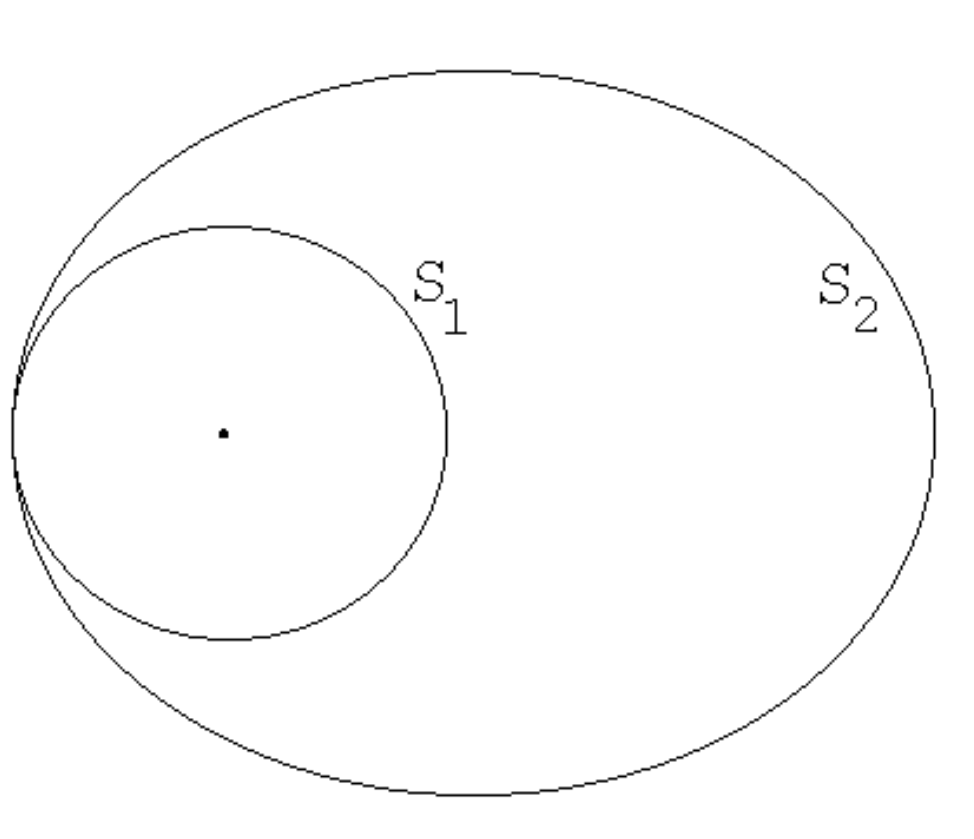
\includegraphics[width=0.6\linewidth]{tutorías/otros/satelites.png}
    \end{figure}


\end{multicols}

\item Una pequeña masa $m$ cae hacie el Sol partiendo del reposo desde una distancia igual al radio de la órbita terrestre. Determine el tiempo de caída usando solo las leyes de Kepler.



% Para imágenes vectoriales -> el texto tiene que estar en LaTeX
% \begin{figure}[htbp]
%   \centering
%   \svgpath{../Imagenes/ejercicios}  -> .. irse pa'trás 
%   \includesvg{ej5.svg}
% \end{figure}

\end{enumerate}
\end{document}
